\documentclass{article}

\usepackage[utf8]{inputenc}
\usepackage[T1]{fontenc}
\usepackage{times}
\usepackage[margin=3cm]{geometry}


% German
%\usepackage[ngerman]{babel}
% English
\usepackage[english]{babel}

\usepackage[round,authoryear]{natbib}
\usepackage{amsmath,amssymb,amsthm}
\usepackage[hyphens]{url}
\usepackage{caption} 
\usepackage{booktabs}
\usepackage{hyperref}
\usepackage{graphicx}
\usepackage{lipsum}

\graphicspath{ {./images} }
\hypersetup{
    colorlinks=true,
    linkcolor=blue,
    filecolor=magenta,      
    urlcolor=blue,
}


% German
%\newtheorem{definition}{Definition}
%\newtheorem{satz}{Satz}
% English
\newtheorem{definition}{Definition}
\newtheorem{theorem}{Theorem}

% TODO
\author{Alexander Lutsch\\Ephraim Siegfried\\Felix Andrist}
\title{ \Huge Cuisinventory }
\date{Fall Semester, 2023 \\ Computer Architecture}


\begin{document}
\maketitle

\section{Cuisinventory Introduction}
Cuisinventory is a grocery inventory managament system offering an easy way to keep track of consumption and additional product information.
It comes in the form of a station which has a barcode scanner and a weight scale with which you can interact. You can scan your groceries' barcode at the Cuisinventory station and
it will automatically fetch related product information like name, brands, allergens and conservation conditions. Additionally you will be able to weigh the groceries and with the fetched information about product quantity,
Cuisinventory will be able to provide percentage information about how much food is left for consumption. All of the inventory information is saved locally in a custom developed database, you can view it on a web application with which the station communicates.

\section{Materials and Software}
\subsection{Hardware}
The following table lists the hardware used to implement the project.
\\[10pt]
\begin{tabular}{l l}
	\hline
	Component              & Model\\
	\hline
	Main Controller        & Adafruit Feather nRF52840\\
	Barcode-Code Scanner   & SparkFun 2D Barcode Scanner Breakout\\
	Strain Gauge Load Cell & Strain Gauge Load Cell - 4 Wires - 5Kg\\
	ADC-Chip               & Adafruit NAU7802 24-Bit ADC - STEMMA QT / Qwiic\\
	Display                & SparkFun LCD-16398\\
	WLAN Co-Processor      & Adafruit AirLift FeatherWing ESP32\\
	I2C Interface          & SparkFun Qwiic / Stemma QT FeatherWing\\
	3 * Buttons            & SparkFun Zubehör Qwiic Button - Green LED\\
	Cable                  & SparkFun Qwiic Cable Kit\\
	Adalogger              & Adalogger FeatherWing - RTC + SD Add-on\\
	Stacking Headers       & Adafruit 12-pin and 16-pin female headers\\
	\hline
\end{tabular} \\[10pt]
Fundamentally we have the main controller, the Adafruit Feather nRF52840, offering a 64MHz ARM Cortex M4F processor along with 256KB of SRAM.
It supports Arduino libraries and has a wide array of external ports to which we can connect the other components.
We expand the capabilties of our main controller with a WLAN Chip and a SD card.
For the interaction with the controller we use 3 main buttons, a strain gauge load cell which measures weight, and a barcode scanner.
A small LCD display outputs information. 
\subsection{Required Libraries}
Conveniently, every required hardware component offered at least one library we could use for the software implementation. 
Below is a table showing the hardware components and a github link to the corresponding libraries we decided for.
\\[10pt]
\begin{tabular}{l l}
	\hline
	Component              & Library\\
	\hline
	Barcode-Scanner        & \href{https://github.com/sparkfun/SparkFun_DE2120_Arduino_Library}{SparkFun DE2120 Arduino Library}\\
	Load Cell \& ADC-Chip  & \href{https://github.com/adafruit/Adafruit_NAU7802}{Adafruit NAU7802}\\
	Display                & \href{https://github.com/sparkfun/SparkFun_SerLCD_Arduino_Library}{SparkFun SerLCD Arduino Library}\\
	WLAN Co-Processor      & \href{https://github.com/adafruit/WiFiNINA}{WiFiNINA Adafruit Fork}\\
	Buttons                & \href{https://github.com/sparkfun/SparkFun_Qwiic_Button_Arduino_Library}{SparkFun Qwiic Button Arduino Library}\\
	Adalogger              & \href{https://github.com/adafruit/SdFat}{SdFat Adafruit Fork}\\
	\hline
\end{tabular} \\[10pt]
Additionally we also rely on the SPI, Wire and SoftwareSerial libraries which are included in the Arduino Core and enable communication protocols for the provided pins of our main controller. \\
On the software side we use the \href{https://github.com/arduino-libraries/ArduinoHttpClient}{Arduino HTTP Client} to help us structure the sending and receiving of HTTP requests.
One of the most important libraries for this project is the \href{https://github.com/bblanchon/ArduinoJson}{Arduino Json Library} with which we can correctly serialize and deserialize JSON Files on our local controller and SD card.
Our database logic fundamentally relies on saving and retrieving information in the JSON format. \\
\subsection{Software Development}
We used git version control to collaborate on the code.
As we weren't happy with the limitations of the Arduino IDE we switched our IDE to PlatformIO.
PlatformIO enabled us a more professional approach. We can define different environments for our compilation and also have automatic library management over a central config file.
With this we can code using external editors and don't have to worry about naming limitations like .ino or different local library versions. Additionally we could implement unit tests for our important classes.

\section{User Manual}
\lipsum[1]\lipsum[1]
\section{Implementation}
\subsection{Hardware}
With a lot of hardware components for this project we had to make sure that we can connect all of them to the microcontroller.
We started with the SD Card extension (Adalogger) and the Wlan Co-Processor. Both of them are small boards about as big as the microcontroller, so using stacking headers we stacked both of them on top of the main controller.\\
\begin{figure}[h]
    \centering
    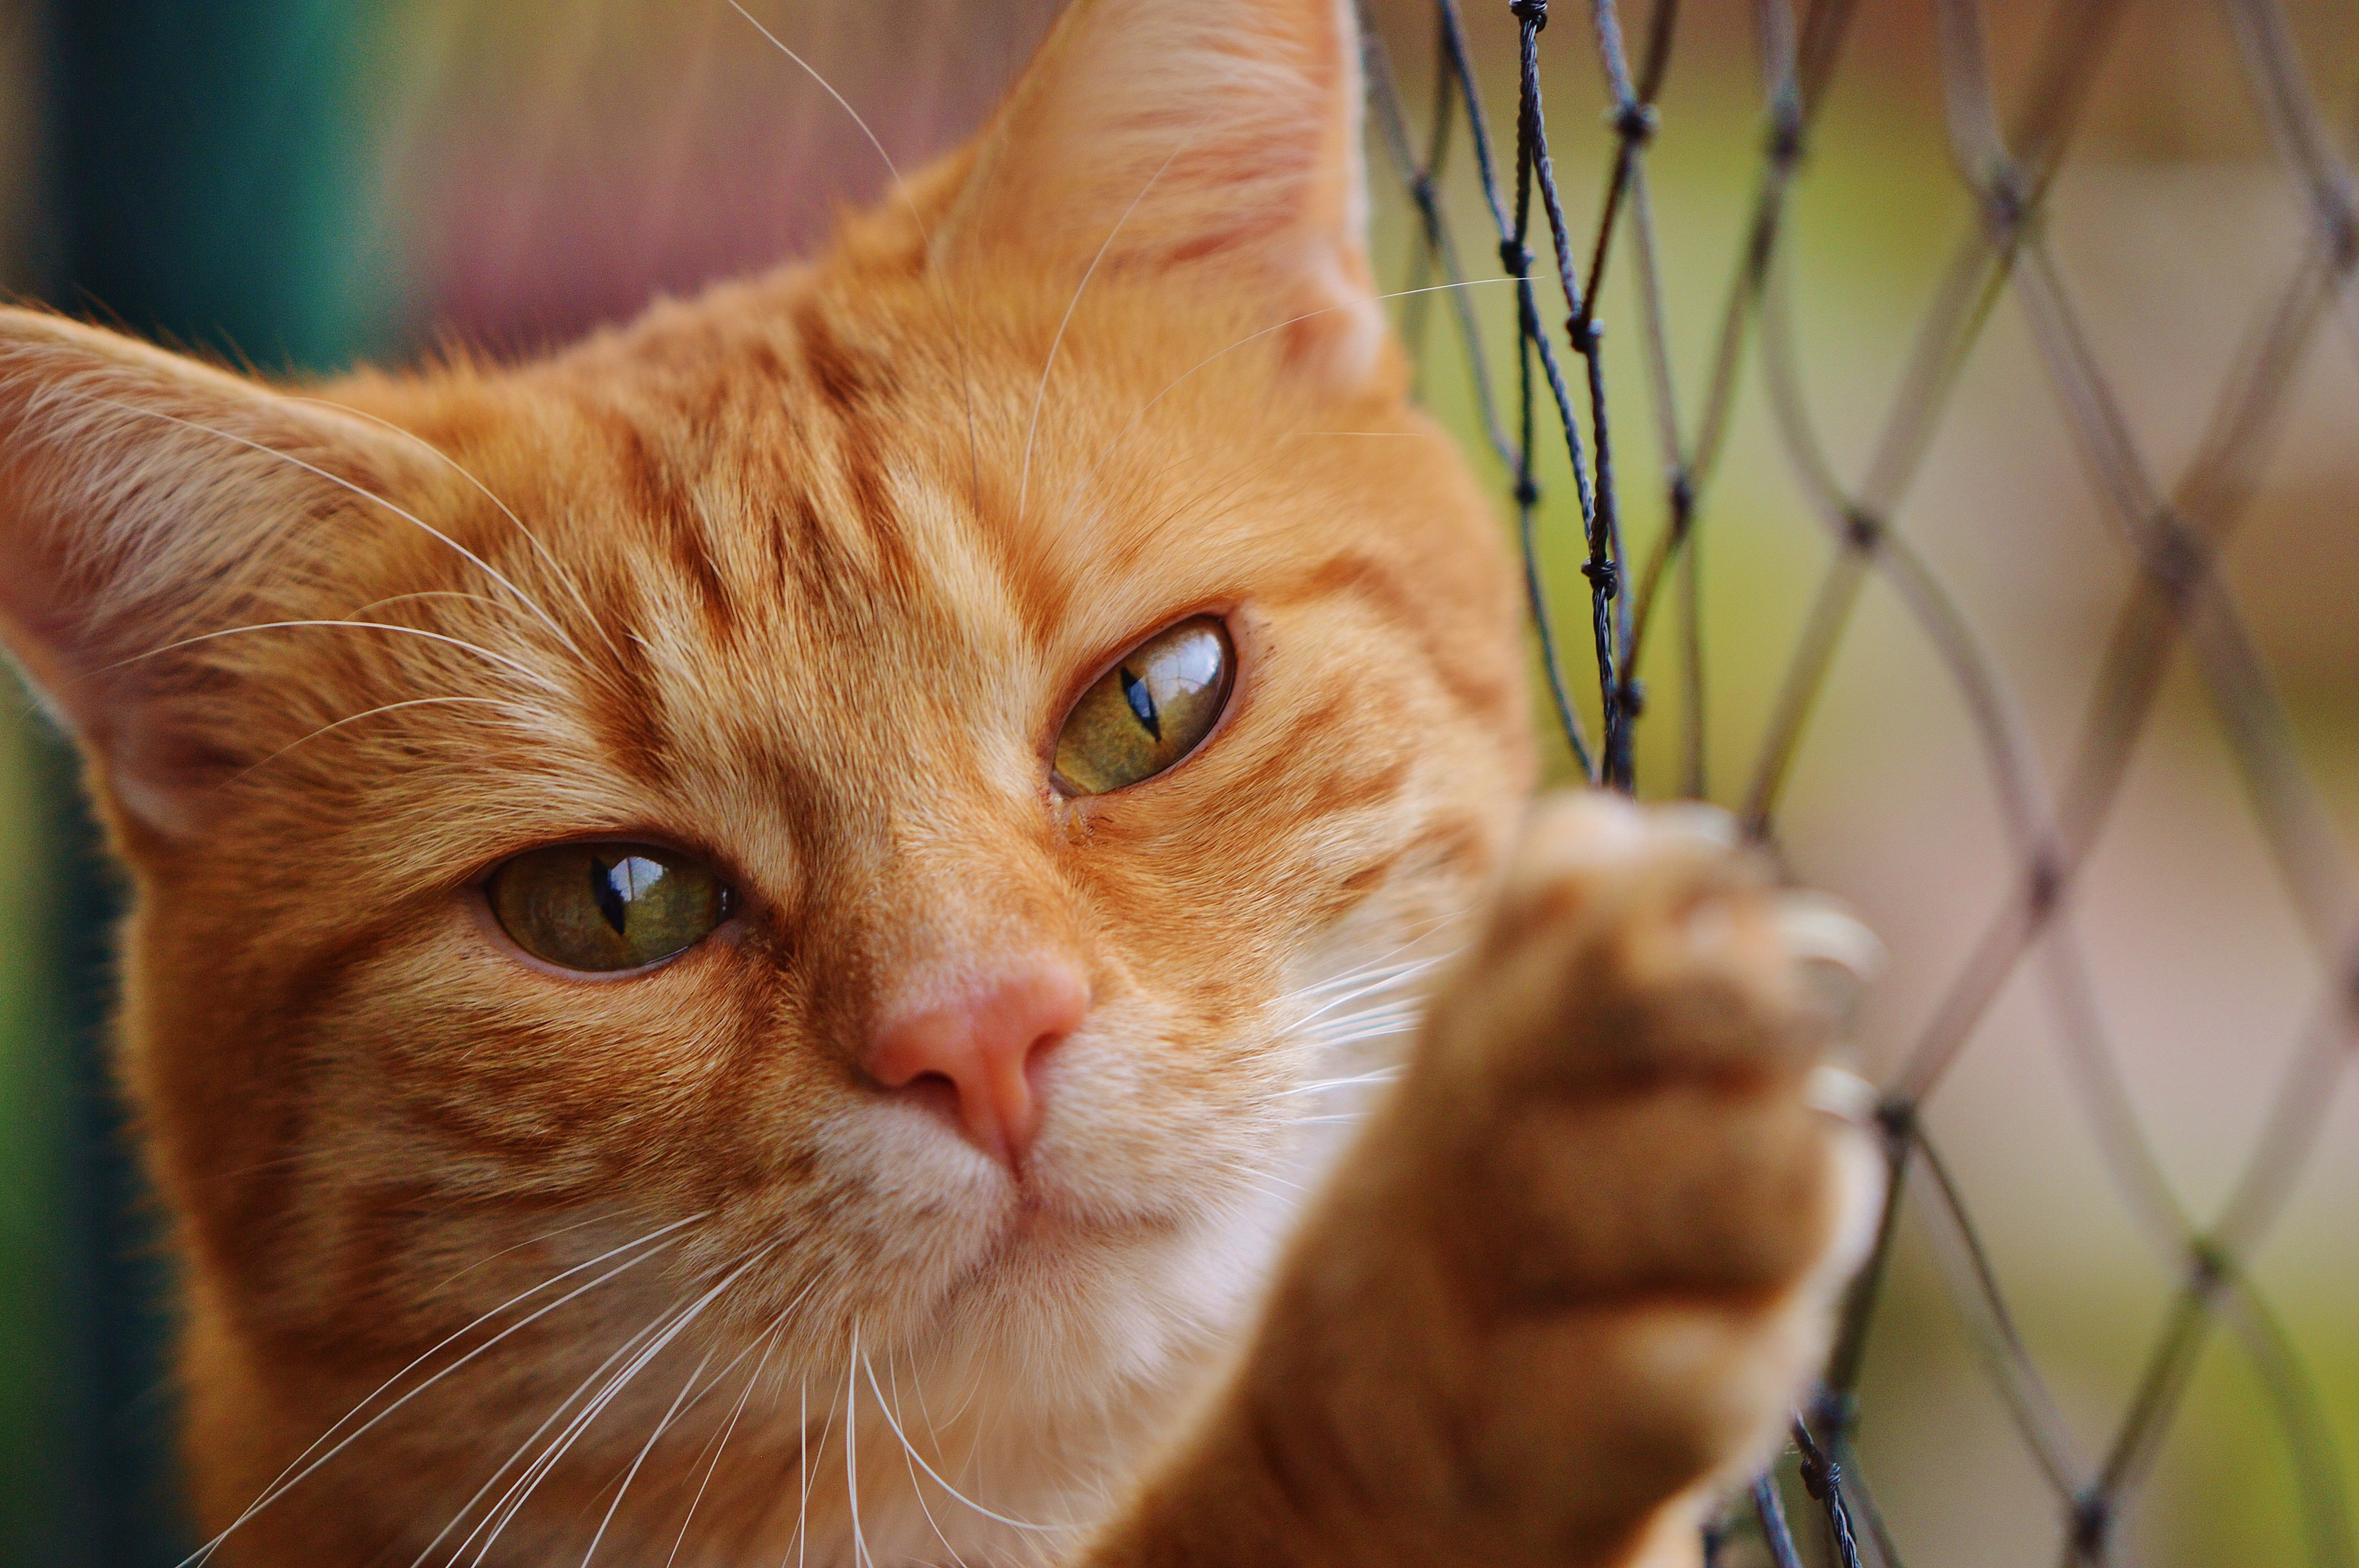
\includegraphics[width=0.5\textwidth]{cat.jpg}
    \caption{Stacking Wifi and SD Card}
    \label{fig:mesh1}
\end{figure}\\
Now whats left is the strain load cell along with the adc chip for weight measurement, the LCD display, the three buttons and the barcode scanner. 
Everything apart from the barcode scanner uses the I2C protocol for communication. This is convenient as I2C supports multiple devices on the same BUS.
We connected the three Buttons, the ADC weight chip and the LCD display over I2C to the same BUS. Additionally we used the SparkFun Qwiic I2C connectors which enable just plugging cables with
connectors together in daisy chain requiring less soldering. The QWIIC connectors required a SparkFun Qwiic Shield board to which we connect the I2C pins and which we again stacked on top of the other boards.\\
This leaves the Barcode Scanner which communicates over UART and still has place on the so far unused RX and TX pins.
With everything connected we just have to check that there is no overlap in the I2C addresses of the devices which are connected to our single I2C Bus.
In our case we had to manually change the I2C addresses of the three buttons over the button software library.
\subsection{Software}

\section{Problems and Solutions}

\section{Summary}

\section{Sources}



\bibliographystyle{apalike}
\bibliography{references}
\end{document}
